% VoyagerMapper quick start — build with: pdflatex quickstart.tex  (run from docs/)
\documentclass[11pt,letterpaper]{article}
\usepackage[margin=0.7in]{geometry}
\usepackage{needspace}
\usepackage{graphicx}
\usepackage[T1]{fontenc}
\usepackage[utf8]{inputenc}
\usepackage{helvet}
\renewcommand{\familydefault}{\sfdefault}
\usepackage{enumitem}
\usepackage{xcolor}
\usepackage{tcolorbox}
\usepackage[hidelinks]{hyperref}
\usepackage{titlesec}
\titleformat{\section}{\large\bfseries}{\thesection.}{0.5em}{}
\titlespacing{\section}{0pt}{14pt}{6pt}
\setlist[enumerate]{leftmargin=*, itemsep=2pt}
\setlist[itemize]{leftmargin=*, itemsep=2pt}
\graphicspath{{img/}}
\definecolor{callout}{RGB}{220,30,30}
\newcommand{\n}[1]{\textcolor{callout}{\textbf{(#1)}}}
\newcommand{\btn}[1]{\textbf{#1}}
\setlength{\parskip}{4pt}
\setlength{\parindent}{0pt}

\begin{document}

{\LARGE\bfseries VoyagerMapper quick start}

\vspace{2pt}
Make a map file for the Trail Tech Voyager Pro in four steps. The default
settings make a file that loads on the device. You do not have to change them.

Start the app with \texttt{run\_gui.bat}. Pan and zoom the map to your riding area.

\section{Select the map and set the opacity}

\begin{center}
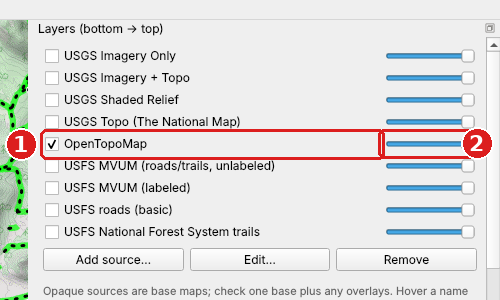
\includegraphics[width=0.78\textwidth]{qs1_layers.png}
\end{center}

\begin{enumerate}
  \item In the \btn{Layers} panel, check the box next to the map you want \n{1}.
        Check one base map, for example \emph{OpenTopoMap} or \emph{USGS Topo}.
        You can also check overlays, for example \emph{USFS MVUM (labeled)}.
  \item Drag the slider at the right of the row to set the opacity \n{2}.
        The map view shows the result at once.
\end{enumerate}

\begin{center}
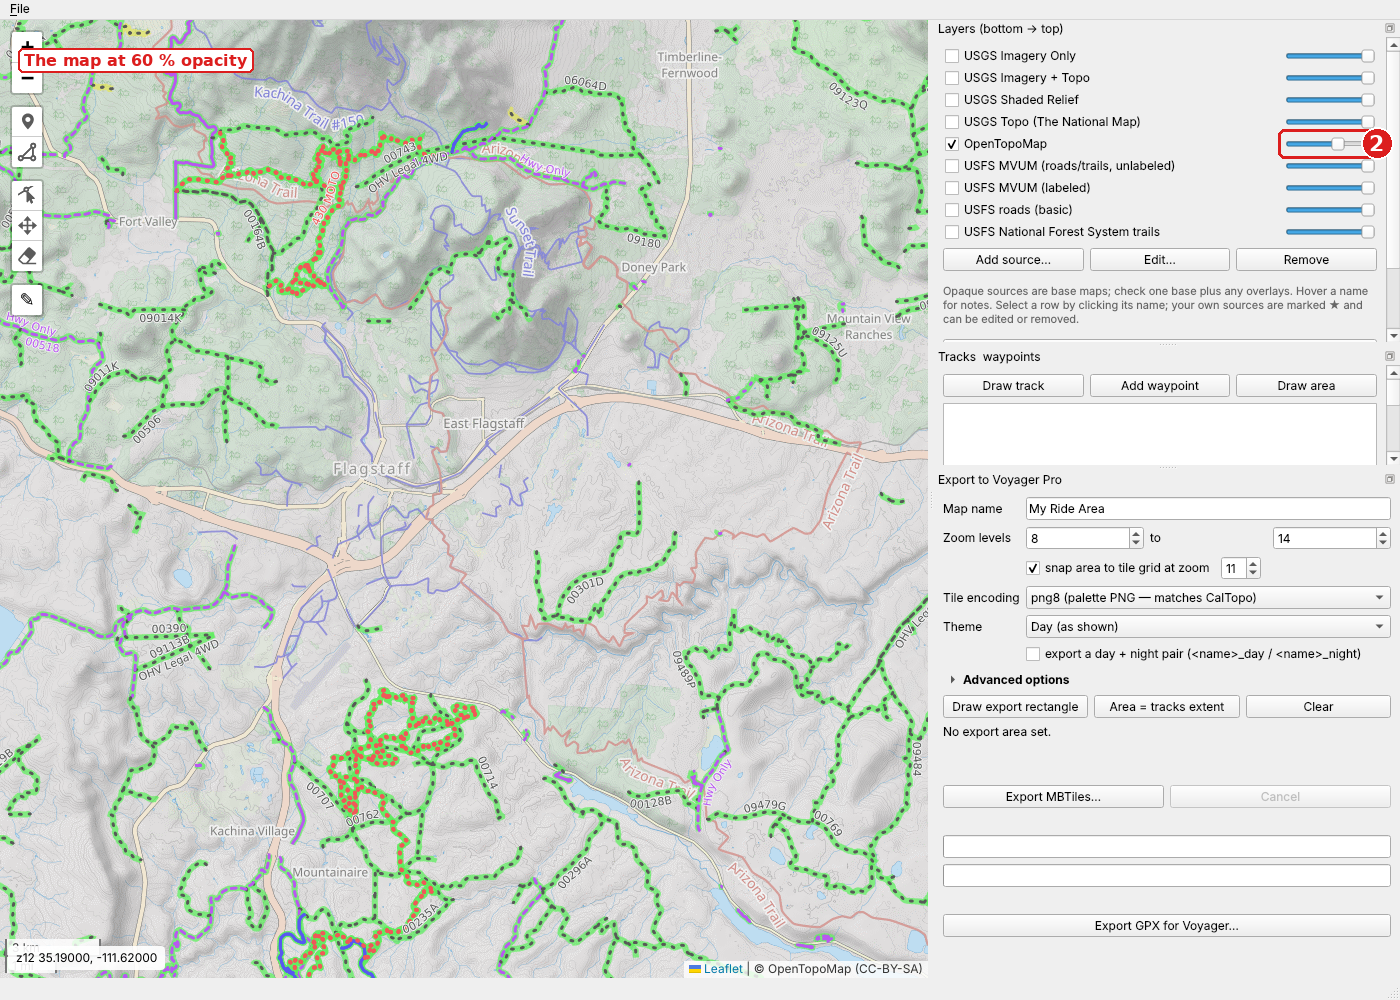
\includegraphics[width=0.9\textwidth]{qs2_opacity.png}
\end{center}

The slider also sets the opacity in the exported file. For a base map, keep the
slider at 100\,\%. Use a lower value for an overlay that hides the base map.

\clearpage
\section{Draw the export area}

\begin{center}
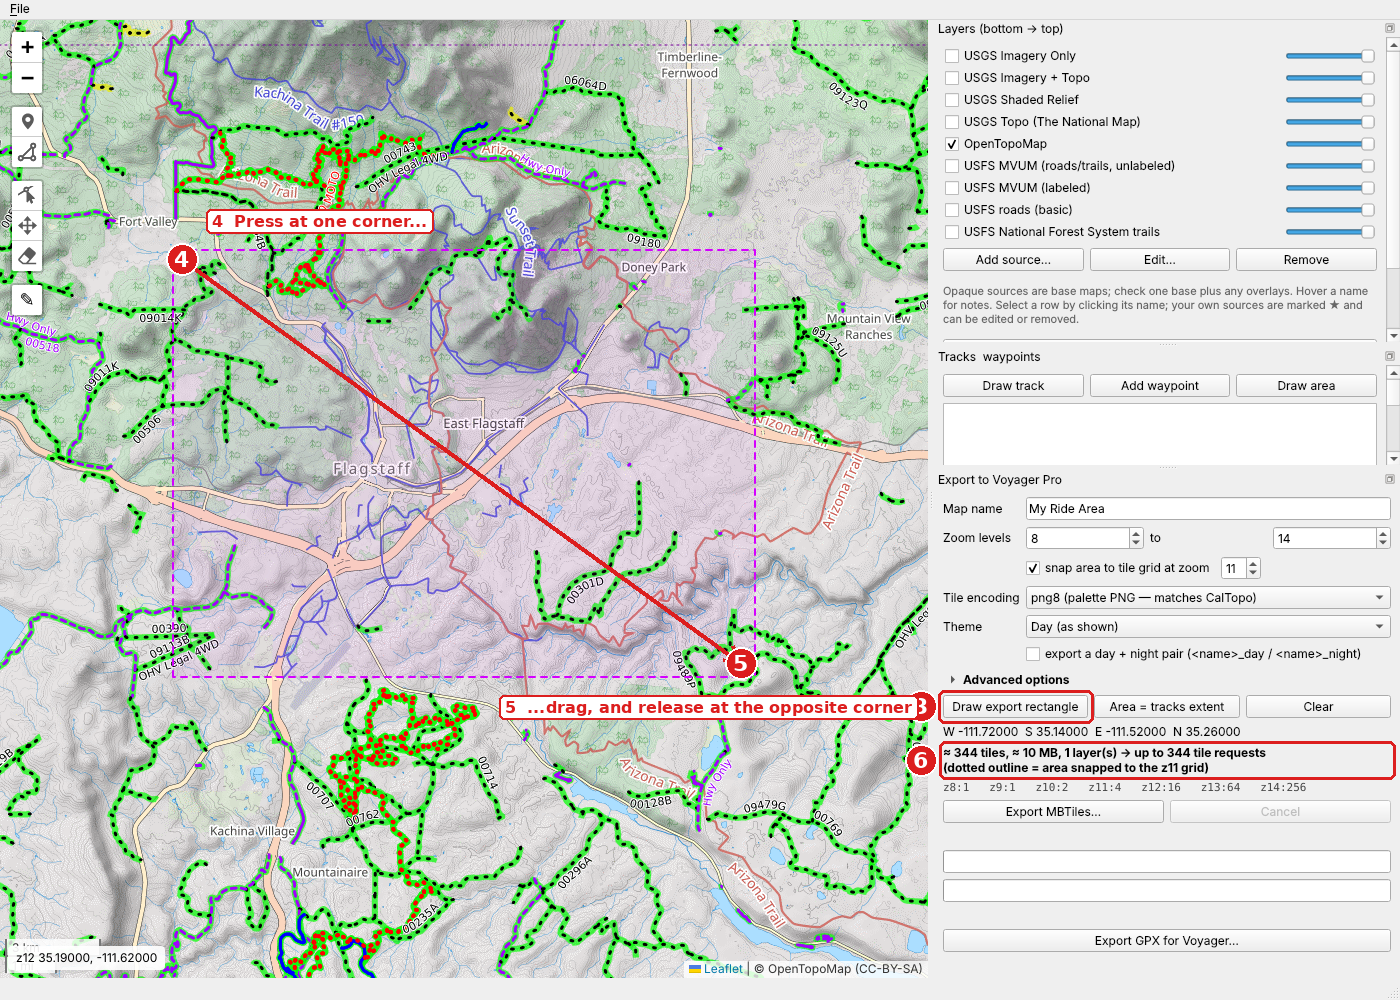
\includegraphics[width=0.95\textwidth]{qs3_area.png}
\end{center}

\begin{enumerate}
  \item In the \btn{Export to Voyager Pro} panel, click \btn{Draw export rectangle} \n{3}.
  \item On the map, press the mouse button at one corner of the area \n{4}.
  \item Hold the button, drag to the opposite corner, and release \n{5}.
\end{enumerate}

The app shows the area as a dashed magenta rectangle. The line under the buttons
shows the tile count and the approximate file size \n{6}. A thin dotted outline
shows the area snapped to the tile grid. That is the area the app exports.

To change the area, click \btn{Draw export rectangle} again and draw a new
rectangle. \btn{Clear} removes the area.

\clearpage
\section{Export the map}

\begin{center}
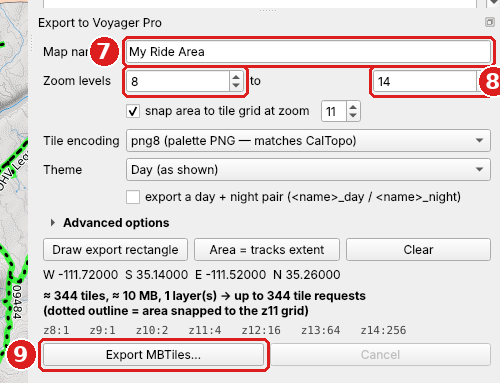
\includegraphics[width=0.62\textwidth]{qs4_export.png}
\end{center}

\begin{enumerate}
  \item Type a name in \btn{Map name} \n{7}. The Voyager Pro shows this name in
        its list of custom maps.
  \item Keep the \btn{Zoom levels} at the default, 8 to 14 \n{8}. More zoom levels
        make a larger file. Each level above 14 makes the file four times larger.
  \item Click \btn{Export MBTiles\ldots} \n{9}.
  \item In the file dialog, choose where to save the \texttt{.mbtiles} file and
        click \btn{Save}.
\end{enumerate}

\begin{center}
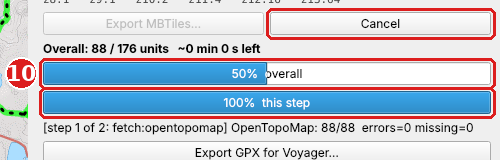
\includegraphics[width=0.62\textwidth]{qs5_progress.png}
\end{center}

The top bar shows the overall progress \n{10}. The bottom bar shows the current
step. The export downloads the tiles for each layer, then writes the file. A
message box opens when the export is complete. \btn{Cancel} stops the export.

\needspace{14\baselineskip}
\section{Load the map on the Voyager Pro}

\begin{enumerate}
  \item Copy the \texttt{.mbtiles} file to the microSD card of the Voyager Pro.
  \item Put the card in the Voyager Pro.
  \item On the device, go to the map screen.
  \item Tap \btn{CUSTOM MAPS}.
  \item Tap \btn{IMPORT A NEW FILE} and select the file.
\end{enumerate}

The device processes the file and shows a message when it is done.

\begin{tcolorbox}[colback=gray!6, colframe=gray!50, title=Tips]
\begin{itemize}
  \item The app keeps the downloaded tiles in a cache. A second export of the
        same area, for example a night version, does not download the tiles again.
  \item Select \btn{Night} in \btn{Theme} to make a dark map. Check
        \btn{export a day + night pair} to make both files in one export.
  \item \btn{File $\rightarrow$ Save project} saves the area, the layers, and the
        export settings, so you can make the same map again later.
\end{itemize}
\end{tcolorbox}

\end{document}
